% ---------- Diagramme de cas d'utilisation ----------
\begin{figure}[!t]
\centering
\begin{tikzpicture}[font=\footnotesize,
  uc/.style={ellipse,draw,align=center,minimum width=3.3cm,minimum height=0.75cm,inner sep=1pt},
  >={Stealth[length=2mm]}]
  \draw (-3.3,0.9) circle (0.15);
  \draw (-3.3,0.75)--(-3.3,0.3) (-3.55,0.6)--(-3.05,0.6)
        (-3.3,0.3)--(-3.5,-0.1) (-3.3,0.3)--(-3.1,-0.1);
  \node at (-3.3,-0.4) {Utilisateur};
  \draw (-2.2,-2.9) rectangle (4.6,2.8);
  \node[anchor=north] at (1.2,2.8) {Programme DE};
  \node[uc] (u1) at (0,2.0) {Choisir la fonction};
  \node[uc] (u2) at (0,0.9) {Choisir Dim et Pop};
  \node[uc] (u3) at (0,-0.3) {Lancer le DE CPU};
  \node[uc] (u4) at (0,-1.6) {Lancer le DE GPU\\(v1, v2 ou v3)};
  \node[uc] (u5) at (3.2,-0.95) {Lire le temps\\et le minimum};
  \foreach \u in {u1,u2,u3,u4} \draw (-3.1,0.5)--(\u.west);
  \draw[->,dashed] (u3.east) -- node[above,font=\tiny,sloped]{$\langle\langle$include$\rangle\rangle$} (u5.north west);
  \draw[->,dashed] (u4.east) -- (u5.south west);
\end{tikzpicture}
\caption{Diagramme de cas d'utilisation. Dim, Pop et la fonction sont fix\'es \`a la compilation (\texttt{make gpu DIM=10 POP=100 OBJ\_FUNC=4}).}
\label{fig:usecase}
\end{figure}

% ---------- Organigramme : un kernel par etape ----------
\begin{figure}[!t]
\centering
\begin{tikzpicture}[font=\fontsize{6}{7}\selectfont,>={Stealth[length=1.5mm]},x=1cm,y=1cm,
  hb/.style={draw,rounded corners=4pt,align=center,minimum width=2.1cm,minimum height=0.55cm,inner sep=1pt},
  kb/.style={draw,align=center,minimum width=3.3cm,minimum height=0.62cm,inner sep=1pt},
  nb/.style={font=\fontsize{4.6}{5.2}\selectfont,text=gray},
  rw/.style={font=\fontsize{5}{6}\selectfont\bfseries}]
  \node[font=\fontsize{6}{7}\selectfont\bfseries,align=center] at (1.1,0.35) {CPU (h\^ote)\\1 thread};
  \node[font=\fontsize{6}{7}\selectfont\bfseries,align=center] at (4.85,0.35) {GPU\\nombre de threads : v2 | v3};
  \draw[dashed,gray] (2.6,0.8) -- (2.6,-9.2);
  \node[draw,fill=gray!25,minimum width=0.4cm,minimum height=7.9cm,inner sep=0] (gm) at (7.75,-4.55) {};
  \node[rotate=-90,font=\fontsize{6}{7}\selectfont\bfseries] at (7.75,-4.55) {M\'emoire globale du GPU};
  % hote
  \node[hb] (init) at (1.1,-0.45) {Allocation\\Copie CPU$\to$GPU};
  \node[draw,diamond,aspect=2.2,inner sep=0pt,align=center] (dec) at (1.1,-3.55) {g\'en\'eration\\$<$ maxGen ?};
  \node[hb] (ret) at (1.1,-8.6) {Copie GPU$\to$CPU\\meilleur individu};
  % kernels
  \node[kb] (ki) at (4.85,-1.15) {\textbf{kernel (I)} hasard (cuRAND)\\[-1pt]\textcolor{gray}{Pop | Pop$\times$D}};
  \node[kb] (ke0) at (4.85,-2.15) {\textbf{kernel (E)} \'evaluation initiale\\[-1pt]\textcolor{gray}{Pop | Pop$\times$D}};
  \node[kb] (kp) at (4.85,-3.55) {\textbf{kernel (P)} tirage de $r_1,r_2,r_3$\\[-1pt]\textcolor{gray}{Pop | Pop}};
  \node[kb] (km) at (4.85,-4.6) {\textbf{kernel (M)} mutation\\[-1pt]\textcolor{gray}{Pop | Pop$\times$D}};
  \node[kb] (kc) at (4.85,-5.65) {\textbf{kernel (C)} croisement\\[-1pt]\textcolor{gray}{Pop | Pop$\times$D}};
  \node[kb] (ke) at (4.85,-6.7) {\textbf{kernel (E)} \'evaluation des essais\\[-1pt]\textcolor{gray}{Pop | Pop$\times$D (+ r\'eduction)}};
  \node[kb] (ks) at (4.85,-7.75) {\textbf{kernel (S)} s\'election\\[-1pt]\textcolor{gray}{Pop | Pop$\times$D}};
  % appels
  \draw[->] (init.south) -- (1.1,-1.15) -- node[pos=0.5,above,rw]{kernel call} (ki.west);
  \draw[->] (1.1,-1.15) -- (1.1,-2.15) -- node[pos=0.5,above,rw]{kernel call} (ke0.west);
  \draw[->] (1.1,-2.15) -- (dec.north);
  \draw[->] (dec.east) -- node[above,rw]{oui} (kp.west);
  \foreach \a/\b in {kp/km,km/kc,kc/ke,ke/ks} \draw[->] (\a.south) -- (\b.north);
  \draw[->] (dec.south) -- node[right,rw,pos=0.1]{non} (ret.north);
  \draw[->] (ks.west) -- (2.35,-7.75) -- (2.35,-2.75) -- (1.1,-2.75);
  \node[rw,align=center,rotate=90] at (2.15,-5.4) {5 kernel calls\\l'un apr\`es l'autre};
  % lectures / ecritures
  \foreach \k in {ki,ke0,kp,km,kc,ke,ks}{
    \draw[<-] ($(\k.east)+(0,0.1)$) -- node[above,rw,pos=0.55]{read} ($(gm.west |- \k.east)+(0,0.1)$);
    \draw[->] ($(\k.east)+(0,-0.1)$) -- node[below,rw,pos=0.55]{write} ($(gm.west |- \k.east)+(0,-0.1)$);
  }
\end{tikzpicture}
\caption{Organigramme du DE massivement parall\`ele avec un kernel par \'etape (versions v2 et v3). En gris, le nombre de threads lanc\'es par chaque kernel. Dans la v1, les kernels (P), (M), (C), (E) et (S) ne forment qu'un seul kernel.}
\label{fig:organigramme}
\end{figure}

% ---------- Repartition des threads ----------
\begin{figure}[!t]
\centering
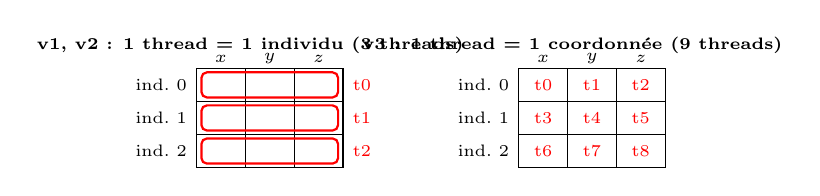
\begin{tikzpicture}[font=\fontsize{6}{7}\selectfont,x=0.62cm,y=0.42cm]
  \foreach \ox/\titre in {0/{v1, v2 : 1 thread = 1 individu (3 threads)},6.6/{v3 : 1 thread = 1 coordonn\'ee (9 threads)}}{
    \node[font=\fontsize{6}{7}\selectfont\bfseries] at (\ox+2.1,1.2) {\titre};
    \foreach \c/\n in {0/x,1/y,2/z} \node at (\ox+1.5+\c,0.8) {$\n$};
    \foreach \i in {0,1,2}{
      \node[anchor=east] at (\ox+1,-\i) {ind.\ \i};
      \foreach \c in {0,1,2} \draw (\ox+1+\c,-\i-0.5) rectangle (\ox+2+\c,-\i+0.5);
    }
  }
  \foreach \i in {0,1,2}{
    \draw[red,thick,rounded corners=2pt] (1.1,-\i-0.38) rectangle (3.9,-\i+0.38);
    \node[red,anchor=west] at (4,-\i) {t\i};
    \foreach \c in {0,1,2}{
      \pgfmathtruncatemacro{\k}{3*\i+\c}
      \node[red] at (8.1+\c,-\i) {t\k};
    }
  }
\end{tikzpicture}
\caption{R\'epartition du travail avec 3 individus et 3 dimensions. Le thread $k$ de la v3 traite l'individu $i=k/D$ et la coordonn\'ee $d=k\bmod D$.}
\label{fig:threads}
\end{figure}
